\usepackage[a4paper,includeheadfoot,left=3cm, right=3cm, top=3cm, bottom=3cm]{geometry}  % margin settings
\usepackage{booktabs}
\usepackage{makecell} % for tables
\usepackage{amsthm}
\makeatletter
\def\thm@space@setup{%
  \thm@preskip=8pt plus 2pt minus 4pt
  \thm@postskip=\thm@preskip
}
\makeatother

\usepackage{hyperref}

%----    define infoboxes    ----%
\usepackage{tcolorbox}
\usepackage{xcolor}

% colors
\definecolor{background}{HTML}{fcfcfc}
\definecolor{tip-text}{HTML}{e7b002}
\definecolor{tip-line}{HTML}{fdce38}
\definecolor{warning-text}{HTML}{b06336}
\definecolor{warning-line}{HTML}{c97d50}
\definecolor{deffun-text}{HTML}{0b797e}
\definecolor{deffun-line}{HTML}{6CC2C9}
\definecolor{design-text}{HTML}{7c972e}
\definecolor{design-line}{HTML}{a7c84a}
\definecolor{trick-text}{HTML}{8c3031}
\definecolor{trick-line}{HTML}{A3595A}

\tcbuselibrary{breakable}
\newtcolorbox{mybox}[1][black]{
  breakable,
  colback=background,
  coltext=black,
  colframe=#1,
  boxsep=5pt,
  arc=4pt}

% tip
\newenvironment{tip}[1][Title]
  {
  \setlength{\fboxsep}{1em}
  \begin{mybox}[tip-line]
    \raisebox{-.2\height}{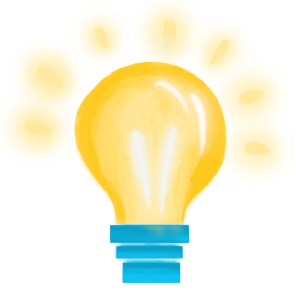
\includegraphics[height=.6cm]{images/lightbulb.png}} \large \textcolor{tip-text}{Consiglio: #1}\\
    }
    {
  \end{mybox}
  }

% warning
\newenvironment{warning}[1][Title]
  {
  \setlength{\fboxsep}{1em}
  \begin{mybox}[warning-line]
    \raisebox{-.2\height}{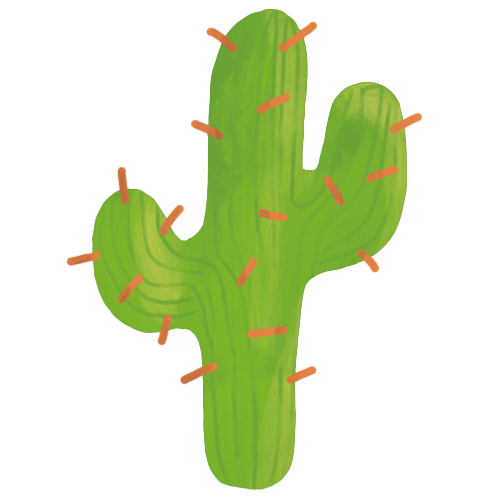
\includegraphics[height=.6cm]{images/gotcha.png}} \large \textcolor{warning-text}{Avvertimento: #1}\\
    }
    {
  \end{mybox}
  }

% deffun
\newenvironment{deffun}[1][Title]
  {
  \setlength{\fboxsep}{1em}
  \begin{mybox}[deffun-line]
    \raisebox{-.2\height}{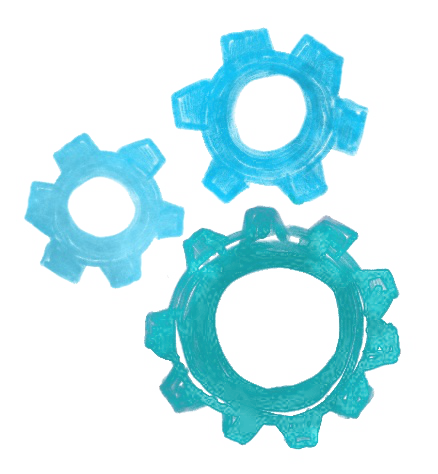
\includegraphics[height=.6cm]{images/gears.png}} \large \textcolor{deffun-text}{Definizione: #1}\\
    }
    {
  \end{mybox}
  }

% design
\newenvironment{design}[1][Title]
  {
  \setlength{\fboxsep}{1em}
  \begin{mybox}[design-line]
    \raisebox{-.2\height}{
\includegraphics[height=.6cm]{images/design.png}} \large \textcolor{design-text}{Approfondimento: #1}\\
    }
    {
  \end{mybox}
  }

% trick
\newenvironment{trick}[1][Title]
  {
  \setlength{\fboxsep}{1em}
  \begin{mybox}[trick-line]
    \raisebox{-.2\height}{
\includegraphics[height=.6cm]{images/hat.png}} \large \textcolor{trick-text}{Trucco: #1}\\
    }
    {
  \end{mybox}
  }

% rinomina tabelle e figure
\renewcommand{\figurename}{Figura}
\renewcommand{\tablename}{Tabella}
